%#! platex thesis.tex

%======================================================================
\chapter{LSTMを用いた手書き医療用語認識とSRP手法及びRatio手法によるデータ拡張}
\label{cha:propose}
本章では,先行研究のBidirectionalLSTMを用いたオンライン手書き医療用語認識を説明する.また,オンライン文字認識用のデータ拡張手法として先行研究のSRP手法を説明し,新手法としてRatio手法を提案する.
%----------------------------------------------------------------------
\section{システムの概要}
\label{sec:concept}
\textbf{図~\ref{sys_concept}} にシステムの概要を示す.提案システムでは,タブレットから収集した手書き医療用語の座標データに対して前処理を行う.その後学習プロセスでは前処理後のデータにSRP手法を用いたデータ拡張を適用し,機械学習における学習データとする.推定プロセスでは,学習を行ったモデルに前処理後のデータを入力し,用語を推定する.

ニューラルネットワーク構造とデータ前処理,特徴量抽出に関しては\ref{ssec:drawing}項の文献\cite{zhang18:drawing}を参考にする.以下,各手順について述べる.

\begin{figure}[tb]
 \begin{center}
  \resizebox{\columnwidth}{!}{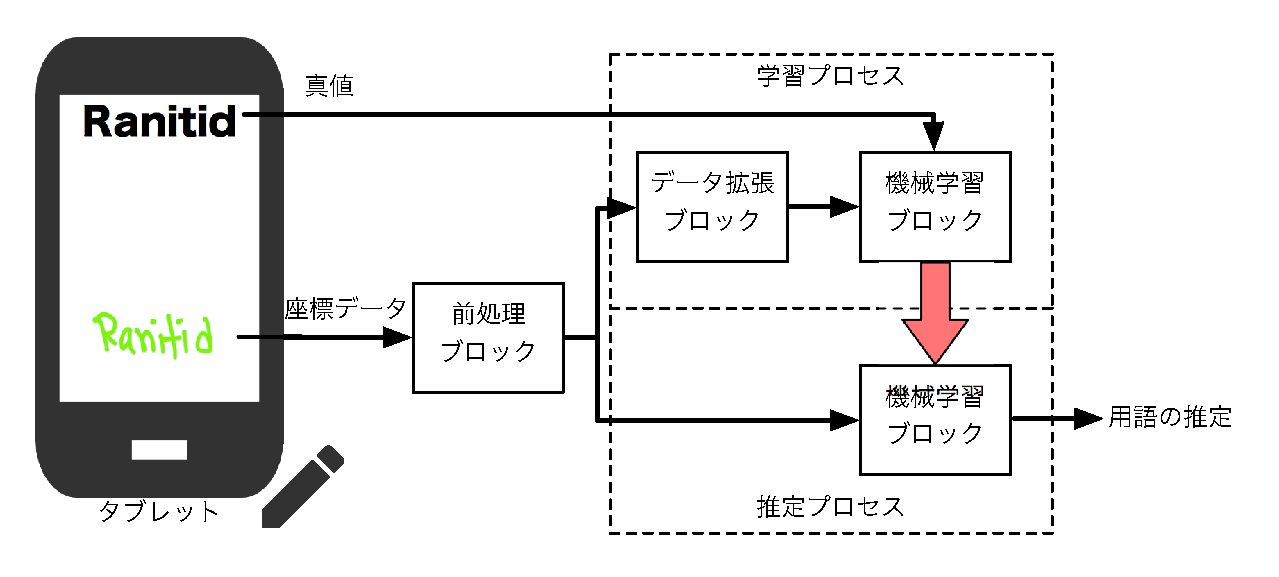
\includegraphics{img/system_structure.eps}}
  \caption{提案システムの概要}
  \label{sys_concept}
\end{center}
\end{figure}

\section{前処理ブロック}
\label{preprocess}
\textbf{図~\ref{preprocess}} に前処理ブロックの概要を示す.前処理ブロックでは,点の除去,正規化,特徴量抽出を行う.直線上の点や近接する点といった,取り除いても文字として成り立つような点の除去を行い,その後正規化を行う.特徴量抽出では点データを直線データへ変換する.以下,前処理ブロックにおける各処理を示す.

\begin{figure}[tb]
 \begin{center}
  \resizebox{\columnwidth}{!}{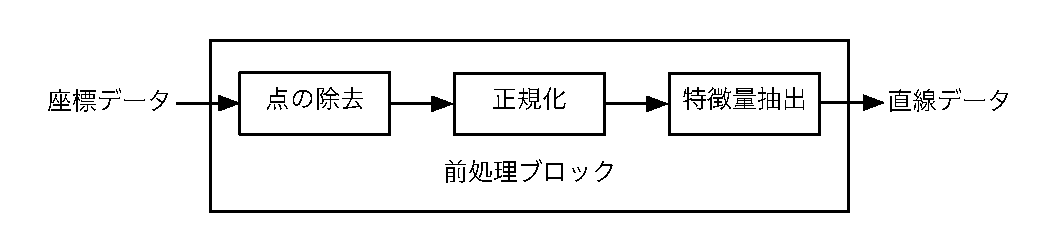
\includegraphics{img/preprocess.eps}}
  \caption{前処理ブロックの概要}
  \label{preprocess}
\end{center}
\end{figure}

\subsection{点の除去}
\label{remove_points}
この処理では,各単語におけるデータの提供者ごとの点の数の差を小さくするため,取り除いても文字として成り立つような点の除去を行う.本研究では直線上の点と近接する点の2種類を除去する.

収穫する医療用語手書きデータは,\textbf{図~\ref{original}}で示したように$(x, y)$座標の時系列データとして存在している.本研究では文献\cite{zhang18:drawing}に従って,これに各点の筆順情報$s$を合わせた$(x, y, s)$を収集する.1つの単語を式~\ref{dataSt}のように収集する.
\begin{equation}
 [[x_1, y_1, s_1], [x_2, y_2, s_2],..., [x_n, y_n, s_n]]
 \label{dataSt}
\end{equation}
$x_i$と$y_i$は点の座標,$s_i$はその点が何画目のストローク上にあるかを示したものである.

手書きデータは書くスピードの違いなどが原因で,同じ単語でもデータ提供者によって点の数が大きく異なってしまい,うまく認識ができない可能性がある.取り除いても文字として成り立つような点の除去を行うことでデータ提供者ごとの点の数の差を小さくすることができる.

本研究で除去する点は2種類ある.1つ目は直線上の点である.\textbf{図~\ref{extra}(a)}に除去する点のイメージ図を示す.点$i$が点$i-1$と点$i+1$の直線上にある場合,点$i-1$から点$i$を通って点$i+1$に向かう線は$i$を除去しても直線として成り立つため,$i$を除去する.$\Delta{x_i}=x_{i+1}-x_i$,$\Delta{y_i}=y_{i+1}-y_i$として式~\ref{eq:cos}を用いてコサインの値を算出し,その値が閾値$T_{cos}$より大きい場合,点$i$を除去する.
\begin{equation}
 \frac{\Delta{x_{i-1}}\Delta{x_i}+\Delta{y_{i-1}}\Delta{y_i}}
 {{(\Delta{x^2_{i-1}}+\Delta{y^2_{i-1}})}^{0.5} {(\Delta{x^2_i}+\Delta{y^2_i})}^{0.5}}
 >T_{cos}
  \label{eq:cos}
\end{equation}
\textbf{図~\ref{extra}(b)}にオリジナルの単語データの例と, \textbf{図~\ref{extra}(c)} に直線上の点が除去された後の単語データの例を示す.

2つ目は近接する点の除去である.\textbf{図~\ref{extra}(a)}にイメージ図を示す.点$i$が点$i-1$と極端に近接している場合,点$i-1$から点$i$を通って$i+1$に向かう線は点$i-1$から点$i+1$までの直線と概ね等しくなるため,点$i$を除去する.直線上の点の除去を行った後,式~\ref{eq:dist}を用いて2点間の距離を算出し,その距離が閾値$T_{dist}$より小さい場合,点$i$を除去する.

\begin{equation}
 \sqrt{(x_i-x_{i-1})^2 + (y_i-y_{i-1})^2} < T_{dist}
  \label{eq:dist}
\end{equation}
\textbf{図~\ref{extra}(d)} に近接する点が除去された後の単語データの例を示す.

\begin{figure}[tb]
 \centering
  \begin{tabular}{c}
    \begin{minipage}[b]{0.5\hsize}
     \centering
     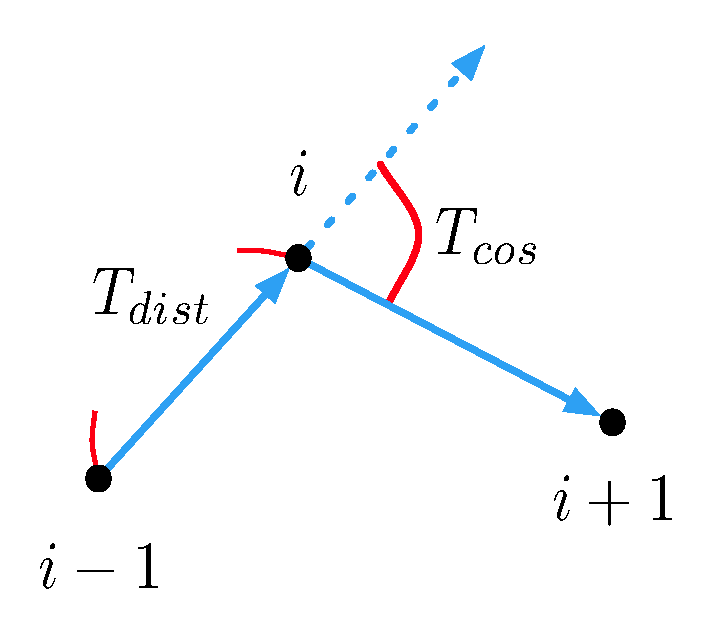
\includegraphics[keepaspectratio,scale=0.5]{img/extraPoint.eps}\\
     (a)イメージ図
    \end{minipage}
   \begin{minipage}[b]{0.5\hsize}
    \centering
    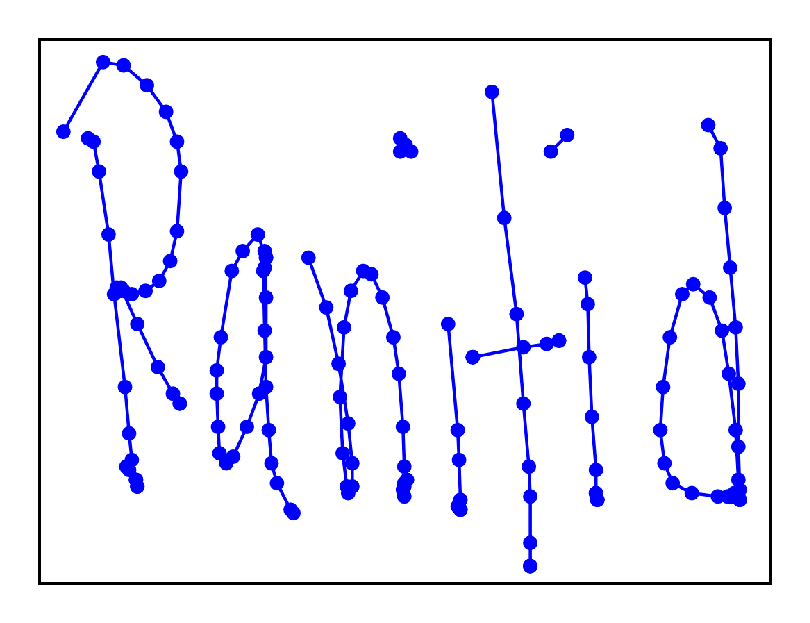
\includegraphics[keepaspectratio,scale=0.5]{img/ranitid.eps}\\
    (b)オリジナルデータ
   \end{minipage}\\
    % \hfill
   \begin{minipage}[b]{0.5\hsize}
    \centering
    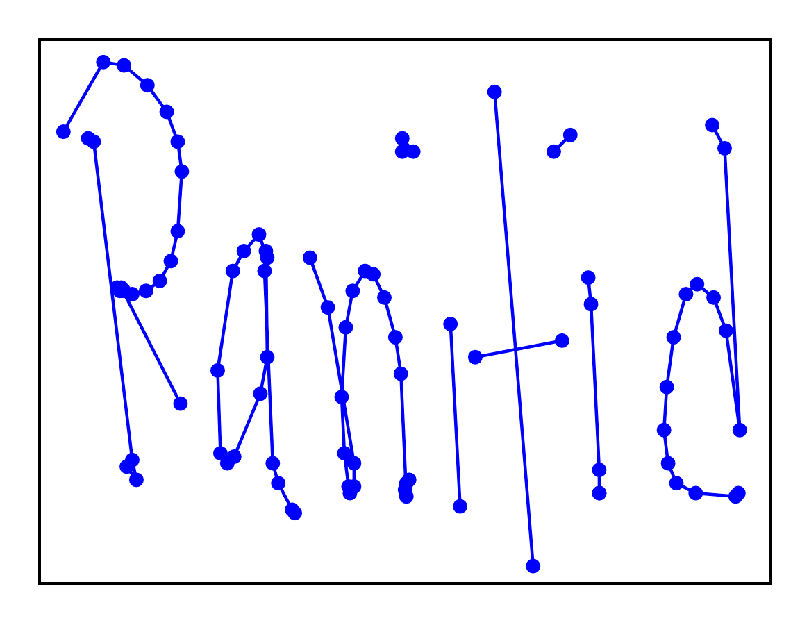
\includegraphics[keepaspectratio,scale=0.5]{img/ranitidStraight.eps}\\
    (c)直線上の点除去後
   \end{minipage}
   \begin{minipage}[b]{0.5\hsize}
    \centering
    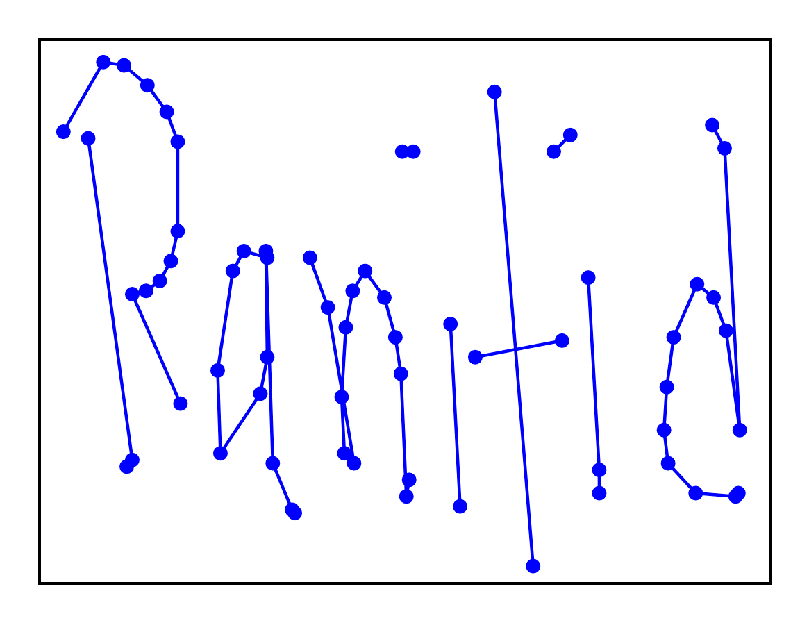
\includegraphics[keepaspectratio,scale=0.5]{img/ranitidClose.eps}\\
    (d)近接する点除去後
   \end{minipage}
  \end{tabular}
 \caption{データ前処理:余分な点の除去}
 \label{extra}
\end{figure}

\subsection{正規化}
\label{normal}
入力データをさらに簡潔にするため,点の除去を施したデータの正規化を行う.
$x$座標について説明する.全てのデータの中から最大値$x_{max}$と最小値$x_{min}$を取り出し,式~\ref{eq:normalize}を用いてある点の$x$座標$X$を$X_{nor}$に正規化する.

\begin{equation}
  X_{nor} = \frac{X - x_{min}}{x_{max}-x_{min}}
  \label{eq:normalize}
\end{equation}
$y$座標に対しても同様の計算を行い,結果的に$(x, y)$をそれぞれ$0$以上$1$以下のデータとする.

\subsection{特徴量抽出}
\label{extract}
機械学習への入力のため,特徴量を抽出する.正規化した点データ2点間を繋ぎ,直線データを作成する.直線データに変換することで,点の座標だけでなく直線の長さ,角度などより多くの特徴量を抽出することができる.線データ$L_i$は,点$i$と点$i+1$から式~\ref{eq:line}のように構成され,本研究ではこのデータを学習における入力データとする.

\begin{equation}
  L_i = [x_i, y_i, \Delta{x_i}, \Delta{y_i}, I(s_i=s_{i+1}), I(s_i \neq s_{i+1})]
  \label{eq:line}
\end{equation}
ここで,$\Delta{x_i}=x_{i+1}-x_i$,$\Delta{y_i}=y_{i+1}-y_i$であり,$I()$は括弧内の条件が真であるときに$1$でありそれ以外では$0$である.

$L_i$において$x_i$と$y_i$は直線の始点を表し,$\Delta{x_i}$と$\Delta{y_i}$は線の始点から終点までの$x$軸方向,$y$軸方向の距離を表す.また$I(s_i=s_{i+1})=1$は,直線の始点と終点が同一ストローク上にあることを示し,$I(s_i \neq s_{i+1})=1$はその直線で次のストロークに移ったことを示す.

\section{データ拡張ブロック}
\label{augment}
様々な手書き文字に対応するため,本研究では多様な提供者から大量のデータを得る必要がある.しかし,十分なデータ量を確保するためには非常に多くの労力と時間を要する.そこで,はじめに先行研究のSRP(Stroke Rotation and Parallel-shift)手法を説明する.その後,文字の縦横比を変更する変更するRatio手法を提案する.これらの手法を用いてデータ拡張を行うことで,手書き文字データの多様性を高める.

\subsection{ストロークの回転}
ストロークの始点と終点の座標から中点を求め,その点を中心にストローク上の点をそれぞれ回転させることでストローク全体を回転させる.この処理を1つのデータに対して複数回施すことで,データ拡張を行う.

\textbf{図~\ref{rotate}(a)}にストロークの回転の原理を示す.ストロークの始点を$(x_f, y_f)$,終点を$(x_l, y_l)$とする.始点と終点の中点を$(a, b)$とすると,式~\ref{eq:center}より$(a, b)$の値が求められる.

\begin{equation}
  (a, b) = (\frac{x_f+x_l}{2}, \frac{y_f+y_l}{2})
  \label{eq:center}
\end{equation}
ストローク上の任意の点の座標を$(x, y)$としたとき,その点を,点$(a, b)$を中心に角$\theta$だけ移動させた後の座標$(X, Y)$は 式~\ref{eq:rotate}で表される.

\begin{equation}
  \left(
    \begin{array}{r}
        X-a \\
        Y-b
    \end{array}
    \right)
 = \left(
  \begin{array}{rr}
      cos\theta & -sin\theta \\
      sin\theta & cos\theta
  \end{array}
  \right)
  \left(
    \begin{array}{r}
        x-a \\
        y-b
    \end{array}
    \right)
  \label{eq:rotate}
\end{equation}
\\

この式をストローク上のすべての点に用いることで,ストローク自体を角$\theta$回転させる.\textbf{図~\ref{rotate}(b)}にストローク回転前の単語データの例,\textbf{図~\ref{rotate}(c)}にストローク回転後の単語データの例を示す.この処理を,ストロークごとに角度を変えながら行うことで元のデータとは異なる形の文字・単語を生成する.それを1つの単語データに対して$N$回行い,データ量を$N$倍に拡張する.

\begin{figure}[tb]
 \centering
  \begin{tabular}{c}
   \begin{minipage}[b]{0.7\hsize}
    \centering
    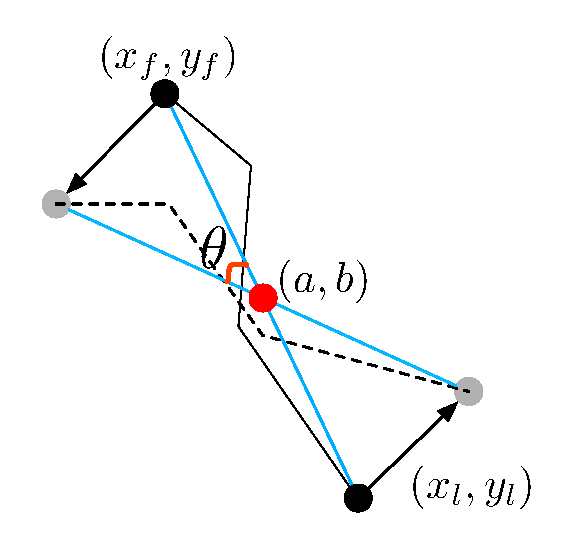
\includegraphics[keepaspectratio,scale=0.7]{img/rotate.eps}\\
    (a)回転の原理
   \end{minipage}\\
    \hfill
   \begin{minipage}[b]{0.5\hsize}
    \centering
    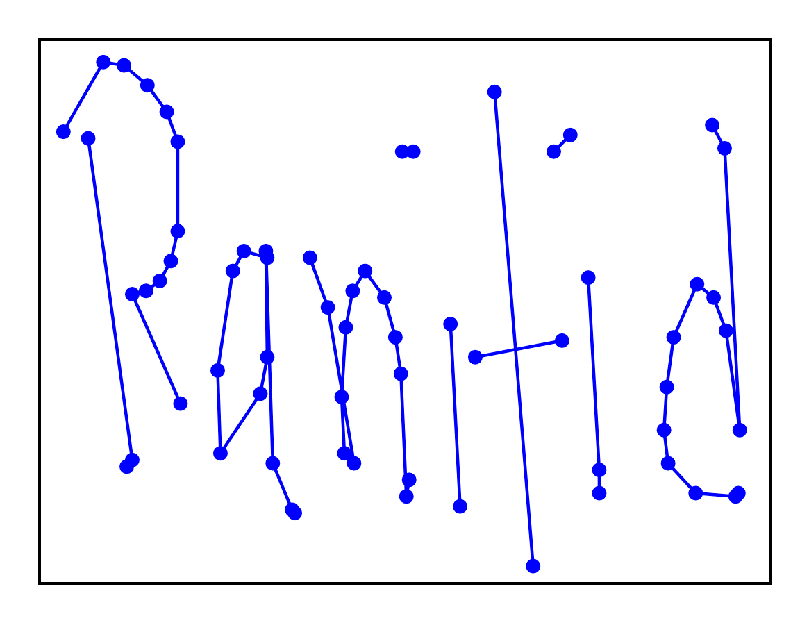
\includegraphics[keepaspectratio,scale=0.5]{img/ranitidCloseBlue.eps}\\
    (b)データ前処理後
   \end{minipage}
   \begin{minipage}[b]{0.5\hsize}
    \centering
    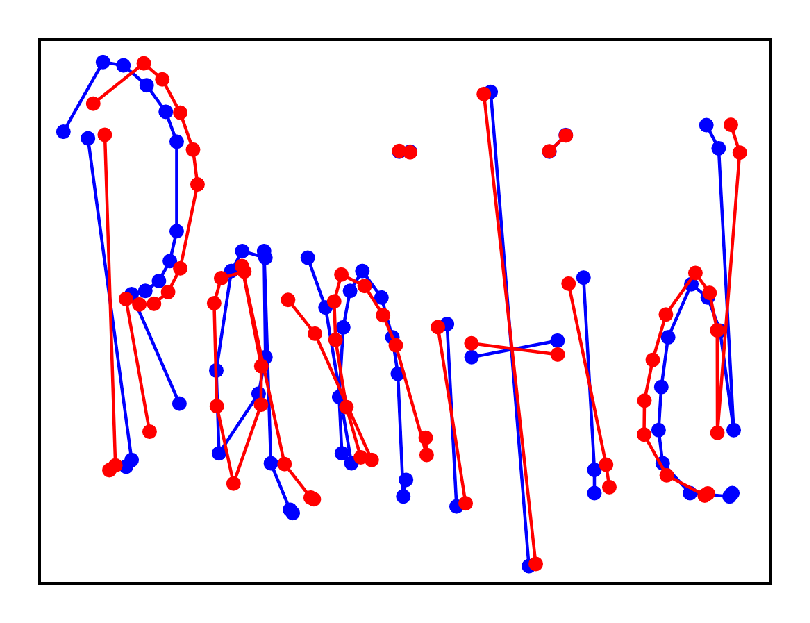
\includegraphics[keepaspectratio,scale=0.5]{img/ranitidRotateRedBlue.eps}\\
    (c)回転前(青)と回転後(赤)
   \end{minipage}
  \end{tabular}
 \caption{ストロークの回転}
 \label{rotate}
\end{figure}

\subsection{ストロークの平行移動}
ストローク上の点の座標それぞれに一定の値を加え,ストローク全体を平行移動させることでデータ拡張を行う.\textbf{図~\ref{parallel}(a)}にストロークの平行移動の原理を示す.ストローク上の任意の点の座標を$(x, y)$としたとき,その点を$x$方向に$dx$,$y$方向に$dy$だけ平行移動させた後の座標$(X, Y)$は 式~\ref{eq:parallel}で表される.

\begin{equation}
  (X, Y) = (x+dx, y+dy)
  \label{eq:parallel}
\end{equation}
この式をストローク上のすべての点に用いることで,ストローク自体を$x$方向に$dx$,$y$方向に$dy$平行移動させる.\textbf{図~\ref{parallel}(b)}にストローク平行移動前の単語データの例,\textbf{図~\ref{parallel}(c)}にストローク平行移動後の単語データの例を示す.この処理を,ストロークごとに$dx$と$dy$の値を変えながら行うことで元のデータとは異なる形の文字・単語を生成する.それを1つの単語データに対して$N$回行い,データ量を$N$倍に拡張する.

\begin{figure}[tb]
 \centering
  \begin{tabular}{c}
   \begin{minipage}[b]{0.7\hsize}
    \centering
    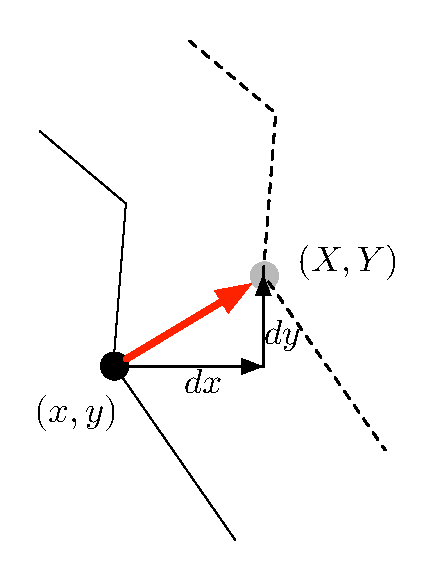
\includegraphics[keepaspectratio,scale=0.7]{img/parallel.eps}\\
    (a)平行移動の原理
   \end{minipage}\\
    \hfill
   \begin{minipage}[b]{0.5\hsize}
    \centering
    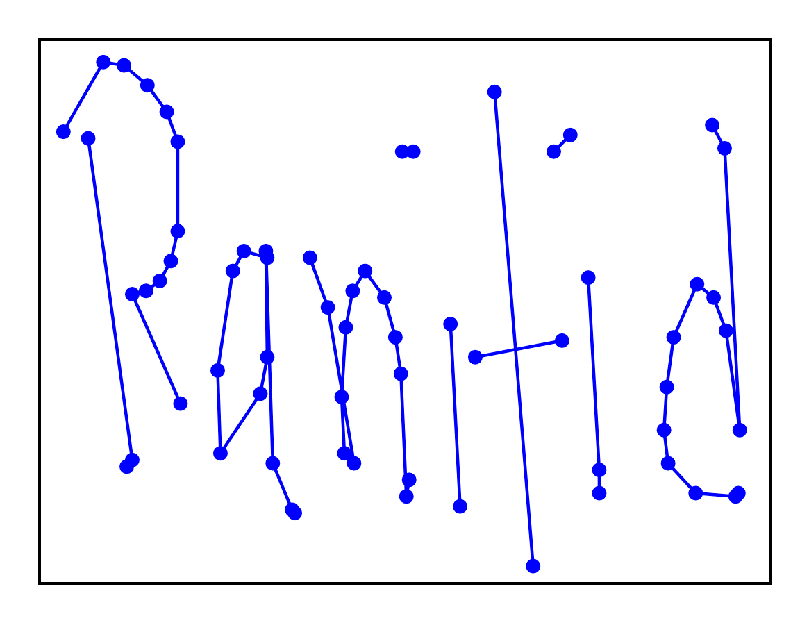
\includegraphics[keepaspectratio,scale=0.5]{img/ranitidCloseBlue.eps}\\
    (b)データ前処理後
   \end{minipage}
   \begin{minipage}[b]{0.5\hsize}
    \centering
    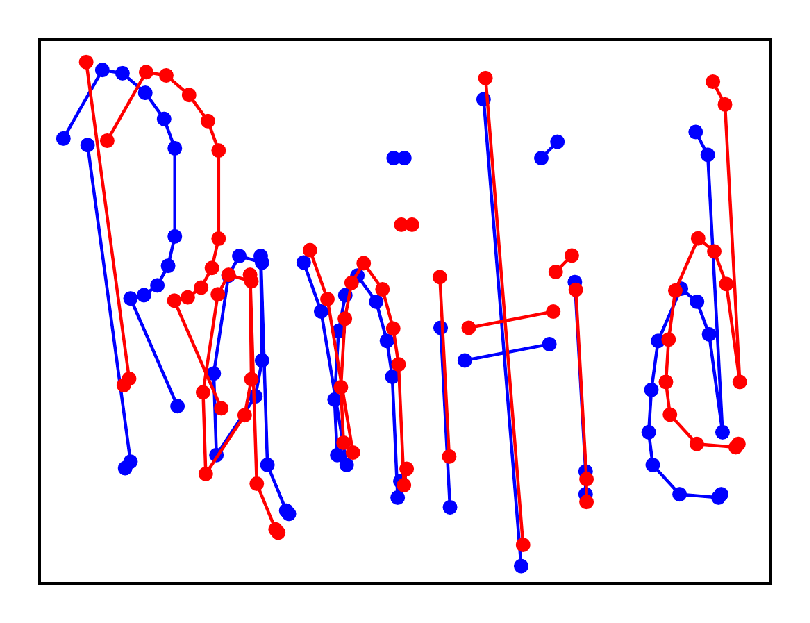
\includegraphics[keepaspectratio,scale=0.5]{img/ranitidParallelRedBlue.eps}\\
    (c)平行移動前(青)と平行移動後(赤)
   \end{minipage}
  \end{tabular}
 \caption{ストロークの平行移動}
 \label{parallel}
\end{figure}




\subsection{文字の縦横比変更}
(まだ全然かけてない,なんとなくで書いておこう)
1つの単語における,すべての点のy座標(もしくはx座標)の平均値を取り,すべての点のy座標(もしくはx座標)に対し(ここになんか書くぞ).\textbf{図}に文字の縦横比変更の原理を示す.
文字の拡張比率を$a$,1つの単語上のすべての点の$y$座標の平均を$\bar{y}$とし,同単語上の任意の点の座標を$(x, y)$としたとき,
その点の$y$座標が$\bar{y}$より大きいときに$y$方向にーーーーーー移動させた後の座標$(X, Y)$は 式~\ref{eq:yratio}で表される.

\begin{equation}
  (X, Y) = (x×1, y×(1+a))
  \label{eq:yratio}
\end{equation}
この式を単語上のすべての点に用いることで,単語全体の点をーーーーーーに移動させる.


.\textbf{図~\ref{yratio}(b)}にストローク平行移動前の単語データの例,\textbf{図~\ref{yratio}(c)}に文字の縦横比率変更後の単語データの例を示す.この処理を,拡張回数ごとに$a$と$x,y$どちらに適応するかをランダムに変えながら行うことで元のデータとは異なる形の文字・単語を生成する.それを1つの単語データに対して$N$回行い,データ量を$N$倍に拡張する.

\begin{figure}[tb]
 \centering
  \begin{tabular}{c}
   \begin{minipage}[b]{0.7\hsize}
    \centering
    %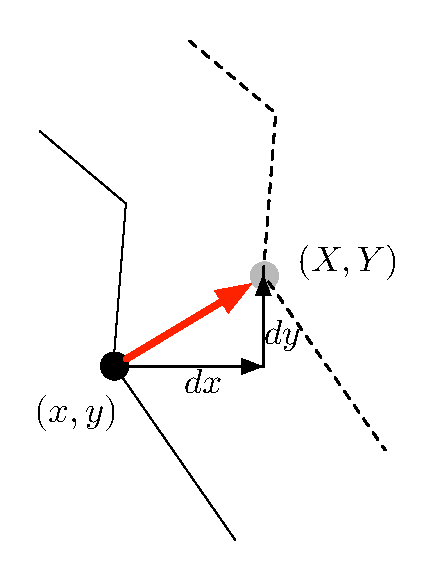
\includegraphics[keepaspectratio,scale=0.7]{img/parallel.eps}\\
    (a)平行移動の原理
   \end{minipage}\\
    \hfill
   \begin{minipage}[b]{0.5\hsize}
    \centering
    %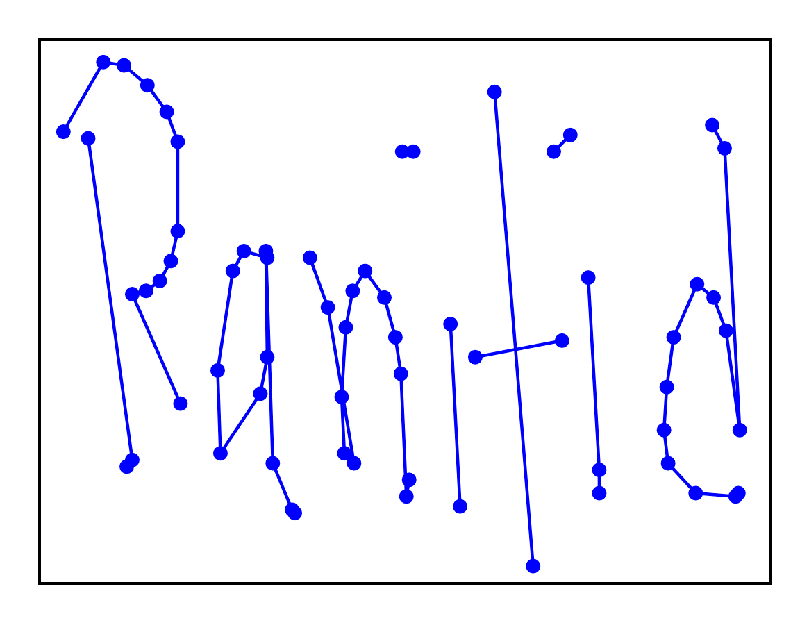
\includegraphics[keepaspectratio,scale=0.5]{img/ranitidCloseBlue.eps}\\
    (b)データ前処理後
   \end{minipage}
   \begin{minipage}[b]{0.5\hsize}
    \centering
    %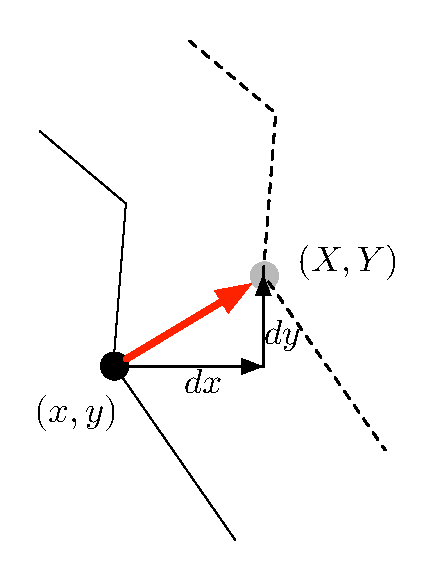
\includegraphics[keepaspectratio,scale=0.5]{img/parallel.eps}\\
    (c)ー移動前(青)とー移動後(赤)
   \end{minipage}
  \end{tabular}
 \caption{ストロークの平行移動}
 \label{yratio}
\end{figure}


\section{機械学習ブロック}
\label{sec:m_learning}
本研究ではBidirectionalLSTMを用いて学習を行う.\textbf{図~\ref{blstm}}にBidirectionalLSTMの概要を示す.BidirectionalLSTMは従来のLSTMに未来の入力から計算を行う逆方向のモデルを加え,出力を同一の出力層に統合するものである.

学習プロセスでは,データ拡張が施された直線データを入力として用いる.本研究においてBidirectionalLSTMは,現在入力されている直線データより前に書かれた直線データだけでなく,後に書かれる直線データも用いて学習を行う.

推定プロセスでは,学習が行われたモデルに前処理後のデータを入力し,用語の推定を行う.

\begin{figure}[tb]
 \begin{center}
  \resizebox{\columnwidth}{!}{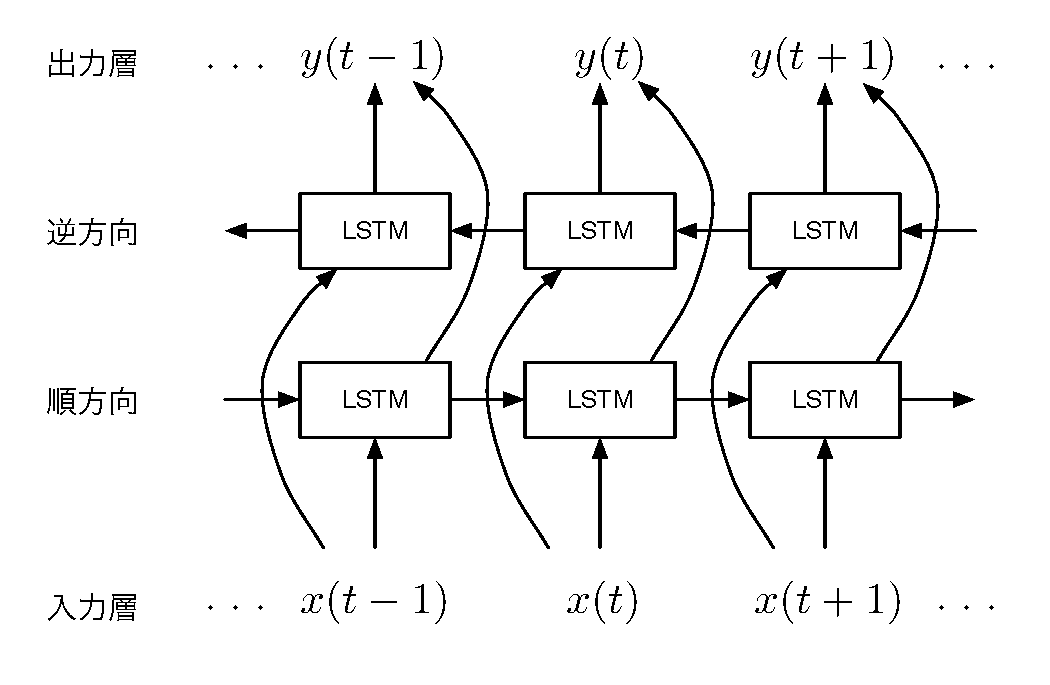
\includegraphics{img/blstm.eps}}
  \caption{BidirectionalLSTMの概要}
  \label{blstm}
\end{center}
\end{figure}

% 以下はRefTeX用
%%% Local Variables:
%%% mode: yatex
%%% TeX-master: "thesis"
%%% End:
